% {\Large \textbf{Mechanical:}}
\qns{Change of Coordinates}
\qcontributor{Yi Zhao, Son Tran, Naomi Sagan, Taejin Hwang}

Many engineering problems can be difficult to solve in its standard xyz coordinates, but may be much easier in a different coordinate system.
In this problem, we will review the process of \emph{change of basis} between coordinate systems.
Remember that a \emph{change of basis} can be represented by a invertible, square matrix.
\par

Let's first start with an example.
Consider the vector $\vec{u} = [u_1, u_2]^T.$ When we write a vector in this form, implicitly we are representing it with the \emph{standard basis} for $\R^{2}$, $\vec{e_1} = [1, 0]^T$ and $\vec{e_2} = [0, 1]^T.$ 

This means that we can write $\vec{u}$ as a linear combination using standard basis vectors $\vec{u} = u_1\vec{e_1} + u_2\vec{e_2}$.
\par

Now, what if we want to represent $\vec{u}$ as a linear combination of another set of basis vectors, say $\vec{a_1} = [1, 1]^T$ and $\vec{a_2} = [0, -1]^T?$
This means that we need to find scalars $u_{a_1}$ and $u_{a_2}$ such that $\vec{u} = u_{a_1}\vec{a_1} + u_{a_2}\vec{a_2}$.
We can write this equation in matrix form:
\[
  \begin{bmatrix}
    | & | \\
    \vec{a_1} & \vec{a_2} \\
    | & |
  \end{bmatrix}
  \begin{bmatrix} u_{a_1} \\ u_{a_2} \end{bmatrix} = \begin{bmatrix} u_{1} \\ u_{2} \end{bmatrix}
.\]
Thus we can find $u_{a_1}$ and $u_{a_2}$ by solving a system of linear equations as seen in 16A.
\par

\meta{
  You can also explain to students that there must be a unique solution, since the U matrix is invertible.
}


\begin{enumerate}
  % Part(a)
  \qitem Let $\vec{v} = [2,-1]^{T}$. What equation gives the coordinates of $\vec{v}$ in the below basis? 
  Try to express your answer in matrix-vector form. No need to do the full calculation.

  \begin{gather*}
    \vec{x} =
    \begin{bmatrix}
      4 \\
      -2
    \end{bmatrix},
    \vec{y} = \begin{bmatrix}
      -3 \\
      -3
    \end{bmatrix}
  \end{gather*}

  % Part(a) solution
  \sol{

    In general, suppose we are given a vector $\vec{u} \in \R^{n}$ in the standard basis and want to change to a different basis with basis vectors $\vec{a_1}, \cdots, \vec{a_n}$.
    If we denote the vector in the new basis as $\vec{u_a} = \begin{bmatrix} u_{a_1} \\ \vdots \\ u_{a_n} \end{bmatrix}$, we solve the following equation $A\vec{u_a} = \vec{u}$, where A is the matrix $\begin{bmatrix} \vec{a_1} & \cdots & \vec{a_n} \end{bmatrix}$.
    Therefore the change of basis is given by:
    \[
      \vec{u_a} = A^{-1}\vec{u}
    .\]

    $$
    \vec{u_a} =
    \begin{bmatrix}
      4 & -3 \\
      -2 & -3
    \end{bmatrix}^{-1}
    \begin{bmatrix}
      2 \\
      -1
    \end{bmatrix}
    $$
  }

  % Part(b)
  \qitem Let $\vec{v} = [3,3]^{T}$. We are told that $\vec{v}$ is represented in the basis:

  \begin{gather*}
    \vec{x} =
    \begin{bmatrix}
      1 \\
      1
    \end{bmatrix},
    \vec{y} = \begin{bmatrix}
      1 \\
      -1
    \end{bmatrix}
  \end{gather*}
  What equation gives the coordinates of $\vec{v}$ in the standard basis?

  % Part(b) solution
  \sol {
    If we already have a vector $\vec{u_a}$ in the basis $\vec{a_1}, \cdots, \vec{a_n}$, how do we change it back to a vector $\vec{u}$ in the standard basis?
    We can reverse the change of basis transformation, thus $\vec{u} = A\vec{u_a}$.
    \par

    $$
    \vec{u_a} =
    \begin{bmatrix}
      1 & 1 \\
      1 & -1
    \end{bmatrix}
    \begin{bmatrix}
      3 \\
      3
    \end{bmatrix}
    $$
  }

 \end{enumerate}

 Now that we've had some mechanical practice, we'll look more into the input-output relationship of vectors.
 For the remaining parts, we'll refer to $[\vec{x}]_S$ or $\vec{x}$ as a vector using standard basis coordinates, and $[\vec{x}]_\beta$ as a vector using $\beta$ basis coordinates.

% Part(c)
 \begin{enumerate}[resume]
  \qitem Let $[\vec{x}]_\beta$ be a vector in $\beta$ coordinates, and $V$ be a change of coordinates matrix from $S \to \beta.$ \\
  How can we represent $\vec{x}$ in terms of $[\vec{x}]_\beta$ and $V?$

  \sol {
    We are given a matrix $V$ that converts standard coordinates to $\beta$ coordinates. 
    This means that $V^{-1}$ will be a matrix that converts $\beta$ coordinates to standard coordinates.
    Therefore, in order to get $\vec{x},$ we multiply $V^{-1}$ with $[\vec{x}]_\beta:$
    $V^{-1} \cdot [\vec{x}]_\beta = [\vec{x}]_S = \vec{x}.$
  }

  % Part(d)
  \qitem Now let $B$ be a linear operator in $\beta$ coordinates. This means that it will take in a vector $[\vec{x}]_\beta$ as an input and output $[\vec{y}]_\beta.$ Given a vector $\vec{x}$ in standard coordinates, why can't we multiply $B \vec{x}$ to get the output $\vec{y}$ in standard coordinates?

  \sol{
    The transformation $B$ "lives" in a different world. It can only accept vectors in $\beta$ coordinates as inputs. 
    Therefore, in order to solve this, we must convert $\vec{x}$ into $\beta$ coordinates.
  }

  % Part(e)
  \qitem Using our $V$ matrix given above, as the change of coordinates matrix from $S \to \beta,$ how can we describe the linear operator $B$ in standard coordinates, that is if $\vec{y} = A \vec{x},$ what is $A$ in the standard basis?

  \sol {
    There will be two main issues we need to address in this question. First off, we need a $\beta$ coordinate input. Secondly, the output of the $B$ is in $\beta$ coordinates, and we will need to convert that back to standard coordinates. 

    Therefore, we take the following steps.

    1. Let's first make our input into $B$ in $\beta$ coordinates. 
    $$\text{Let } \vec{v} = V \vec{x}.$$
    2. Now if we input $\vec{v}$ we will get some output:
    $$\vec{w} = B \vec{v}.$$
    3. However, $\vec{w}$ is in $\beta$ coordinates, so we must convert back to standard coordinates using $V^{-1}.$
    $$\vec{y} = V^{-1} \vec{w}$$
    4. Cascading all of our matrix multiplications, we end up with:
    $$\vec{y} = V^{-1} B V \vec{x}.$$
    Therefore, we can see that $A = V^{-1} B V.$

    The following can also be represented in this state diagram: 

    Note that when cascading transformations, we apply them to the \textbf{left} of the existing transformation.

    \begin{figure}[H]
      \centering
      \begin{tikzpicture}[node distance = 2cm, thick]%
        \node (1) {$\vec{x}$};
        \node (2) [right=of 1] {$\vec{y}$};
        \node (3) [below=of 2] {$\vec{w}$};
        \node (4) [below=of 1] {$\vec{v}$};
        \draw[->] (1) -- node [midway,above] {$A$} (2);
        \draw[->] (1.240) -- node [midway,left]{$V$} (4.120);
        \draw[->] (4.60) -- node [midway,right]{$V^{-1}$} (1.300);
        \draw[->] (2.300) -- node [midway,right]{$V$} (3.60);
        \draw[->] (3.120) -- node [midway,left]{$V^{-1}$} (2.240);
        \draw[->] (4) -- node [midway,below] {$B$} (3);
      \end{tikzpicture}%
    \end{figure}
  }
  % % Part(c) solution
  % \sol{
  %   Start by writing $\vec{x_1}$ in terms of $\vec{z_1}$:
  %   $$ \vec{x_1} = V \vec{z_1} $$
  %   Then, apply the transformation $A$ to $\vec{x_1}$, substituting $V \vec{z_1}$ for $\vec{x_1}$:
  %   $$ \vec{x_2} = A V \vec{x_1} $$
  %   Finally, left-multiply both sides by $V^{-1}$ to change $\vec{x_2}$ to the eigenbasis:
  %   $$ \vec{z_2} = V^{-1} \vec{x_2} = V^{-1} A V \vec{z_1} $$

  %   $$A' = V^{-1} A V =
  %   \begin{bmatrix}
  %     1 & 1 \\
  %     -2 & 1
  %   \end{bmatrix}^{-1}
  %   \begin{bmatrix}
  %     3 & -1 \\
  %     -2 & 4
  %   \end{bmatrix}
  %   \begin{bmatrix}
  %     1 & 1 \\
  %     -2 & 1
  %   \end{bmatrix}
  %   $$

  %   $A'$ represents the transformation $A$ in the eigenbasis of $A$, so we know that $A'$ is the diagonal matrix:
  %   $$ A' =
  %   \begin{bmatrix}
  %     \lambda_1 & 0 \\
  %     0 & \lambda_2
  %   \end{bmatrix} =
  %   \begin{bmatrix}
  %     5 & 0 \\
  %     0 & 2
  %   \end{bmatrix} $$

  %   In general, suppose we have a linear transformation $T$ represented by a $n \times n$ matrix that transforms $\vec{u} \in \R^{n}$ to $\vec{v} \in \R^{n}$:
  %   \[
  %     \vec{v} = T\vec{u}
  %   .\]
  %   Suppose we have a basis vectors $\vec{a_1}, \cdots, \vec{a_n} \in \R^{n}$, and the vectors $\vec{u}, \vec{v}$ above are represented in this basis:
  %   \[
  %     \begin{aligned}
  %       \vec{u_a} &= u_{a_1}\vec{a_1} + \cdots + u_{a_n}\vec{a_n} \\
  %       \vec{v_a} &= v_{a_1}\vec{a_1} + \cdots + v_{a_n}\vec{a_n}.
  %     \end{aligned}
  %   \]
  %   Thus we have
  %   \[
  %     \begin{aligned}
  %       T\vec{u}          &= \vec{v} \\
  %       TA\vec{u_a}       &= A\vec{v_a} \\
  %       A^{-1}TA\vec{u_a} &= \vec{v_a}.
  %     \end{aligned}
  %   \]
  %   By pattern matching, we see that if we set $T_a = A^{-1}TA$, we get the relationship $T_a\vec{u_a} = \vec{v_a}$ in the new basis.
  %   The correspondences stated above are all represented in the following diagram:
  %   % \begin{figure}[H]
  %   %   \centering
  %   %   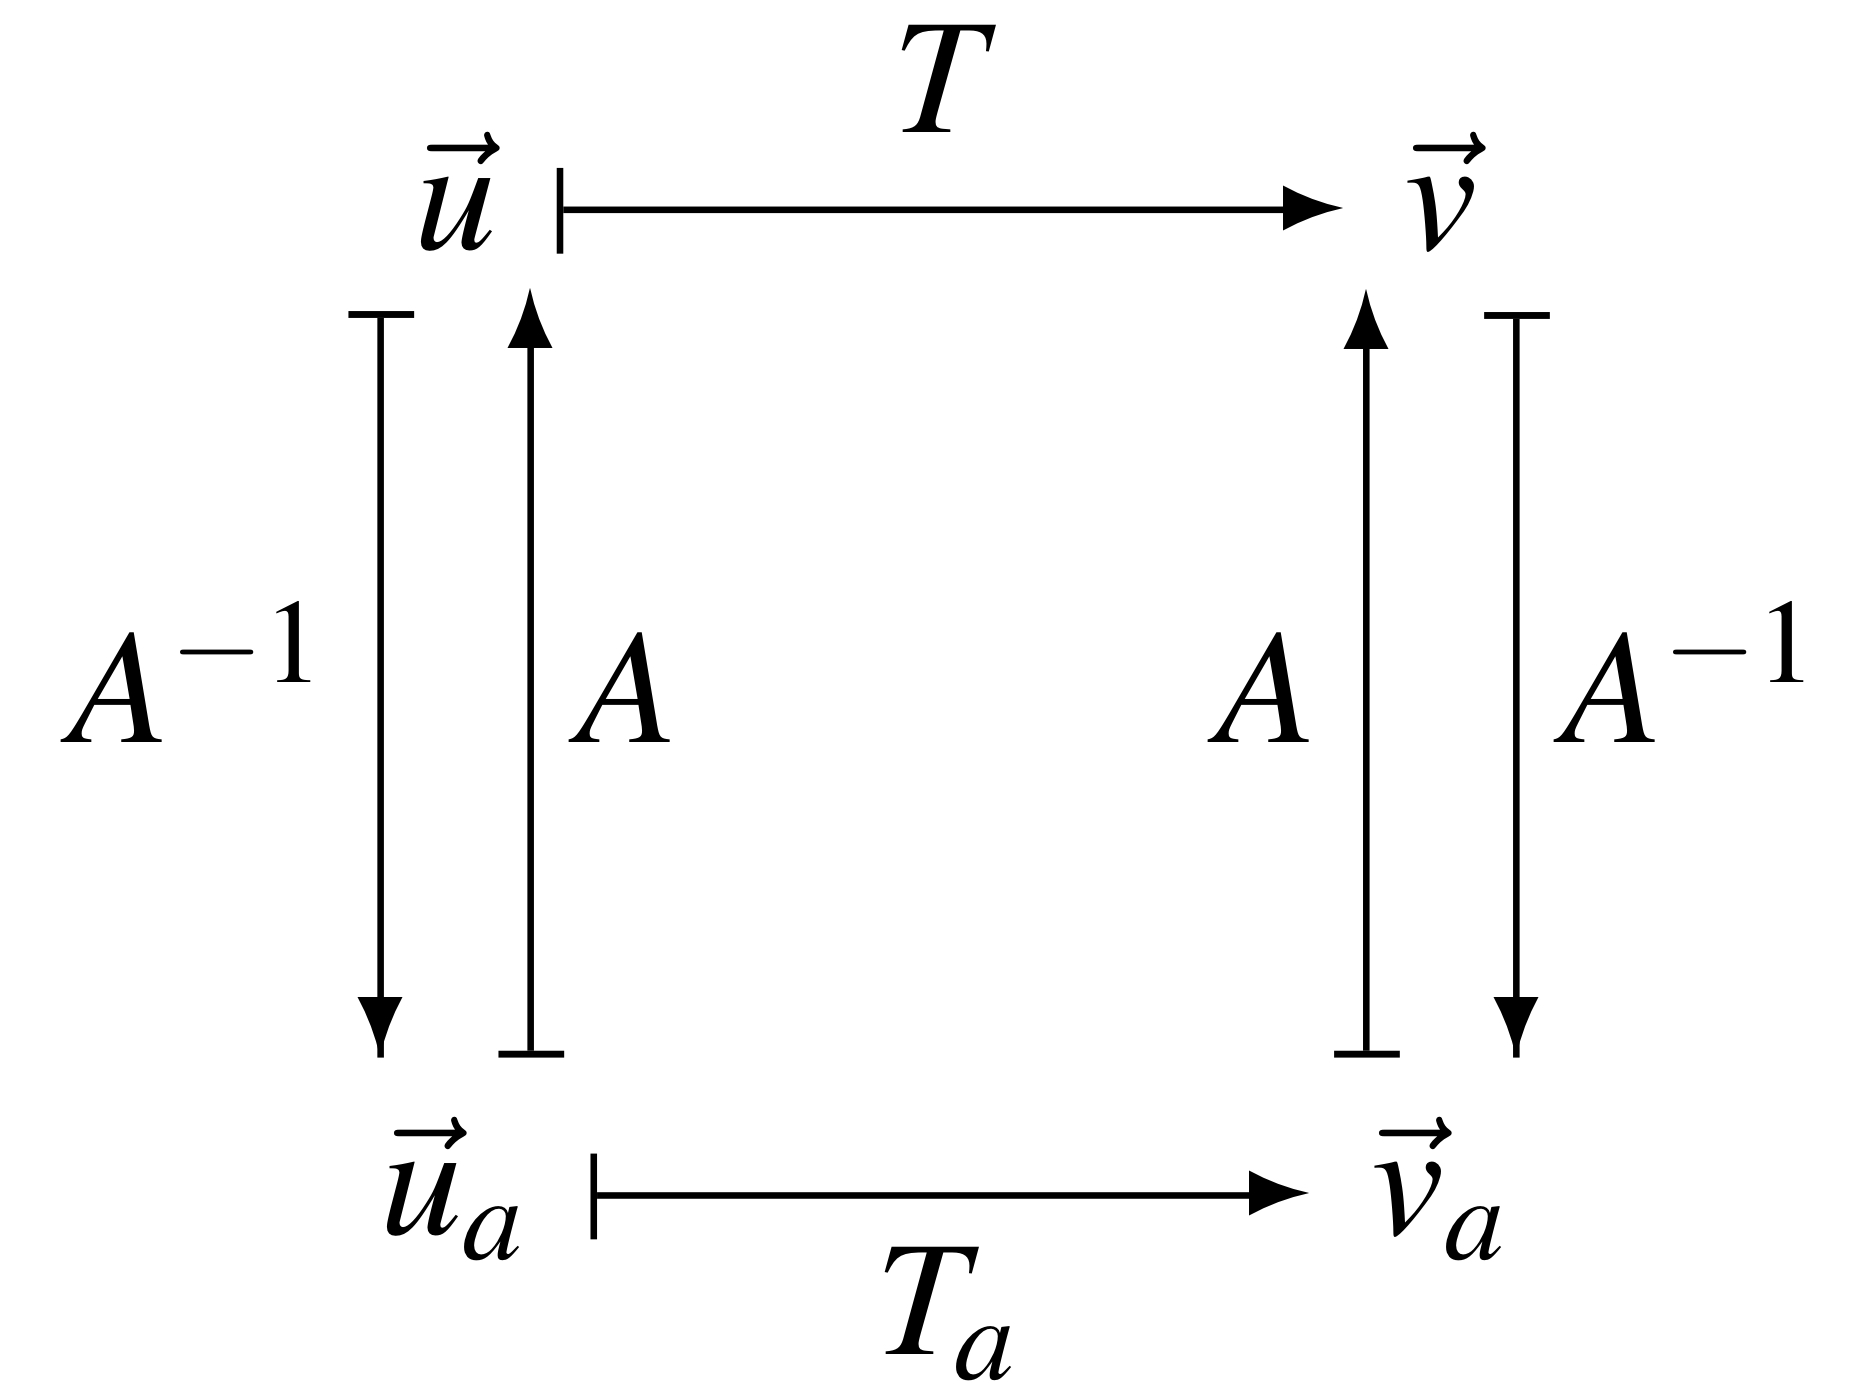
\includegraphics[scale=0.1]{\bank/statespace/figures/change_of_basis.jpg}
  %   % \end{figure}
\end{enumerate}
